\label{sec:slope_diff_piezo}
Другой метод, предложенный авторами \cite{piezo50}, заключается в измерении интенсивности
дифрагированного образцом излучения при фиксированной отсройке от точного
брэговского угла кристалла образца в двухкристальной геометрии.
% Необходимо  встать в произвольную точку на кривой дифракционного отражения,
% другими словами выведем интенсивность детектора из максимума отражения в точку на склоне
%  кривой (Рис.~\ref{ris:kdopiez}).

\begin{figure}[H]
\centering
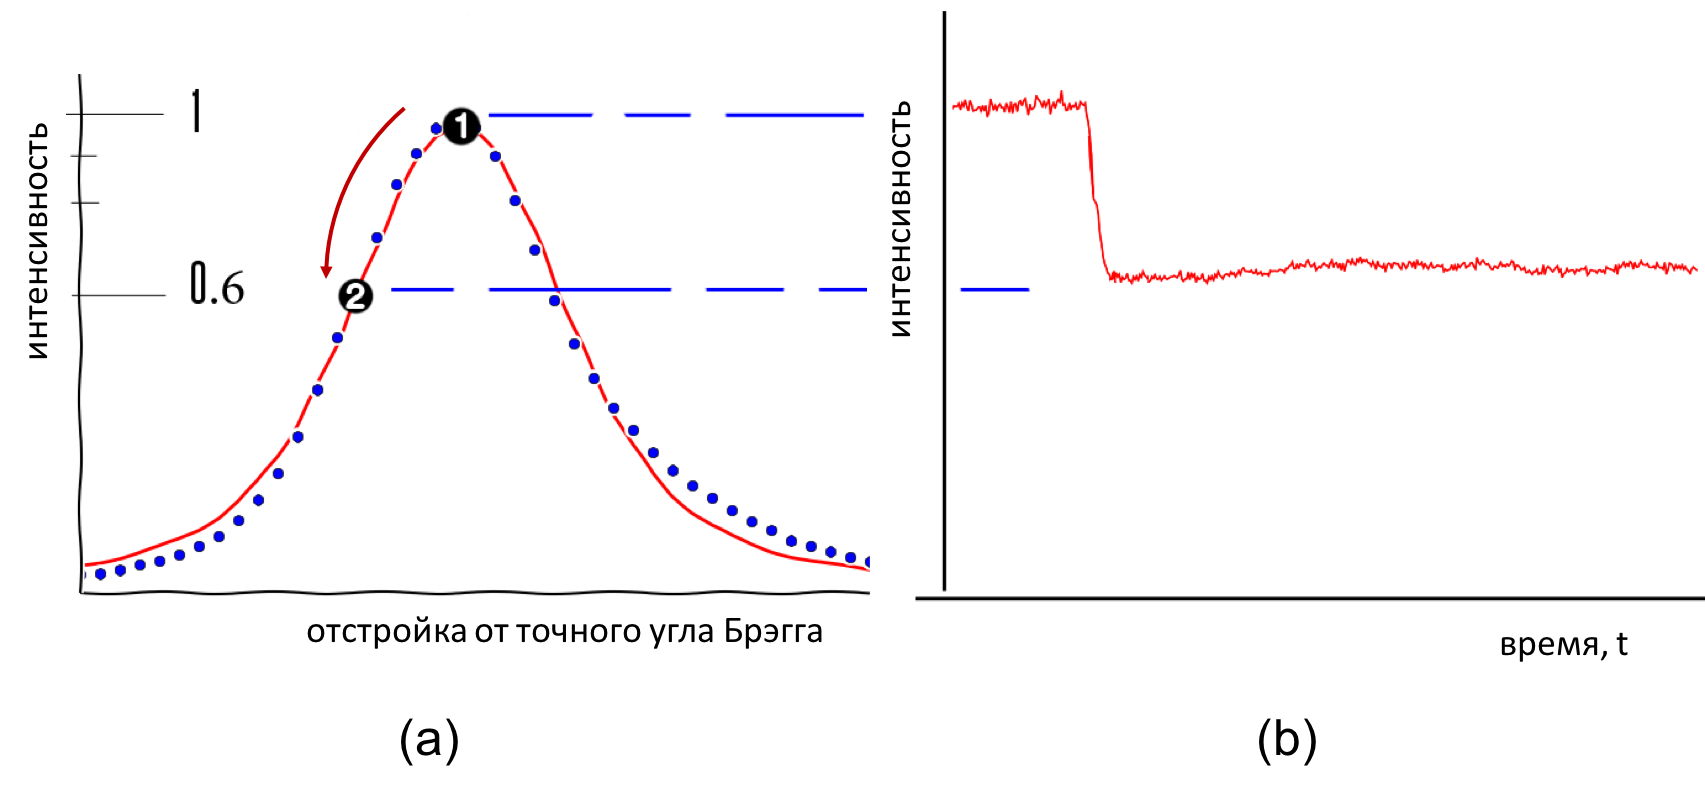
\includegraphics[width=1\linewidth]{images/kdopiez2.png}
\caption{Отстройка кристалла из точного брэгговского положения в положение,
соответствующее склону КДО (а) и соответствующее изменение интенсивности сигнала на детекторе (b)}
\label{ris:kdopiez}
\end{figure}
\noindent
Другими словами, необходимо выставить образец в угловое положение, соответсвующее склону КДО.
В таком случае, при смещении КДО в результате пьзоэффекта будет наблюдаться резкое изменение
интенсивности при неподвижном образце, т.е при таком подходе даже не требуется проводить
измерение КДО, зная точно ее форму и скачок интенсивности вызванный внешним воздействием.
Несмотря на то, что данный подход позволяет существенно улучшить временное разрешение метода,
он применим лишь для тех случаев, когда профиль КДО не изменяется под воздействием поля.

\begin{figure}[H]
\centering
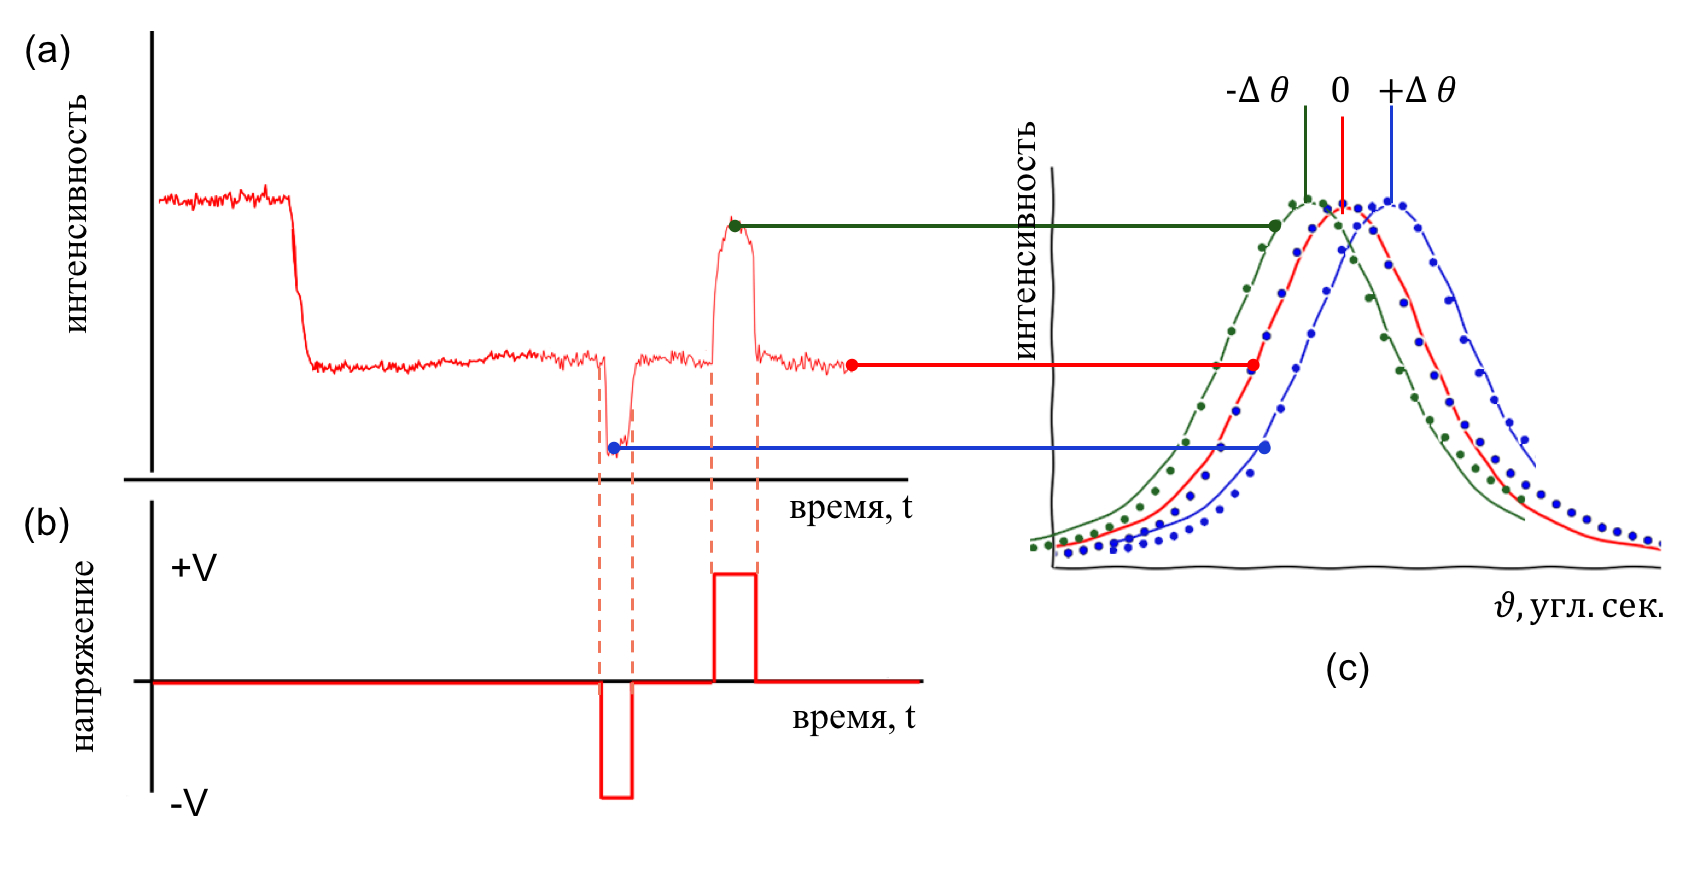
\includegraphics[width=0.8\linewidth]{images/princip2.png}
\caption{Интенсивность сигнала на детекторе (a); величина  приложенного напряжения к
поверхности кристалла (b); восстановленное положение КДО (c)}
\label{ris:princip}
\end{figure}

Из рис. \ref{ris:princip}  видно, что время, за которое деформируется кристалл
в результате пьезоэффекта, много меньше разрешающей способности даже данного метода.
